% !TeX spellcheck = en_GB
% Methods text

\section{Database: AudioSet}

\subsection{What is AudioSet} \todo{How cite?}

	Audio Set can be described as a sound large-scale dataset that has the intention of putting the availability of audio and image data on the same level. It is composed by a huge variety of manually-annotated audio events and is organized by following an important ontology formed by 632 different audio classes. The data has been extracted from YouTube videos and the labelling process has been based on diverse factors such as metadata, context and content analysis. It has been developed by Google with the purpose of producing an audio event recognizer that can be applied to plenty of acoustic situations coming from the real world \cite{Gemmeke2017}.
	
\subsection{Ontology}

	In order to put this dataset together the events have been organized in an abstract hierarchy. This is composed by higher-level classes which  describe a certain type of sound and also acts as parents of other labels that refer to more specific events. With this purpose, the relationship among different classes needed to be non-exclusive, so labelling similar audio events may result into a more general class, the parent, if there existed ambiguity. This is also helpful for labellers due to group the clips in an easier and faster way.
	
	The Audio Set Ontology has been made considering some fundamental guidelines as the ones explained below:
	% List
	% !TeX spellcheck = en_GB
\begin{itemize}
	\item \doubt{A complete collection of all labels must be prepared} so that it can be used to define sound events from real-world aural data.
	\item When labelling an audio event the result must match the criteria of a common listener.
	\item Different categories should be easy to distinguish by an ordinary listener. In the case that two different labels do not satisfy this requirement, these should be merged. With this condition, the spectrum of possible labels remains limited.
	\item The distinction of two different classes must be done by relying just on the audio, it cannot be accompanied by image or visual information.
	\item The hierarchy should not be very deep by keeping the number of children per parent class to no more than 10. This also eases the annotation labour. 
\end{itemize}

	
	It is easy that an ontology of this volume gets leaned or biased in a particular direction due to several factors, such as the subjectiveness of its creators or the selection of the initial set of classes used when starting to work. With the intention of generating a primary list that covers a wide range of audio events in an objective way, the researchers decided to apply an impartial, web-scale text analysis from the very beginning. They agreed on detecting hyponyms of the word "sound" by utilizing a modified version of the famous technique called \textit{Hearst patterns} \cite{Hearst1992}, a method proposed to automatically acquire hyponymy lexical relations from unrestricted text. As a result, an enormous collection of terms came up. This was filtered by considering how well these terms represented audio, i.e. by combining together the global frequency of occurrence and how exclusively these are recognized as hyponyms of "sound" instead of other terms. As an output of the final process, a list of 3000 terms was obtained.
	
	With respect to the hierarchical relation among categories, it was constructed by the authors with the main intention that this satisfied their human comprehension of the sounds. Event though this is a subjective manner, it also makes sense since this is how the hierarchy best performs its labour on helping human labelling.
	After all the organization process, the model is not based on a strict behaviour as a singular node can appear in many different locations, i.e., a single node can be child of different parent nodes. The final result is composed by 632 audio event labels and, in the hierarchy, there is no deeper case than 6 levels. Figure \ref{fig:mesh1} shows the nodes that belong to the two top layers of the ontology.
	
	% Figure of ontology
	\begin{figure}[h]
		\centering
		\captionsetup{justification=centering}
		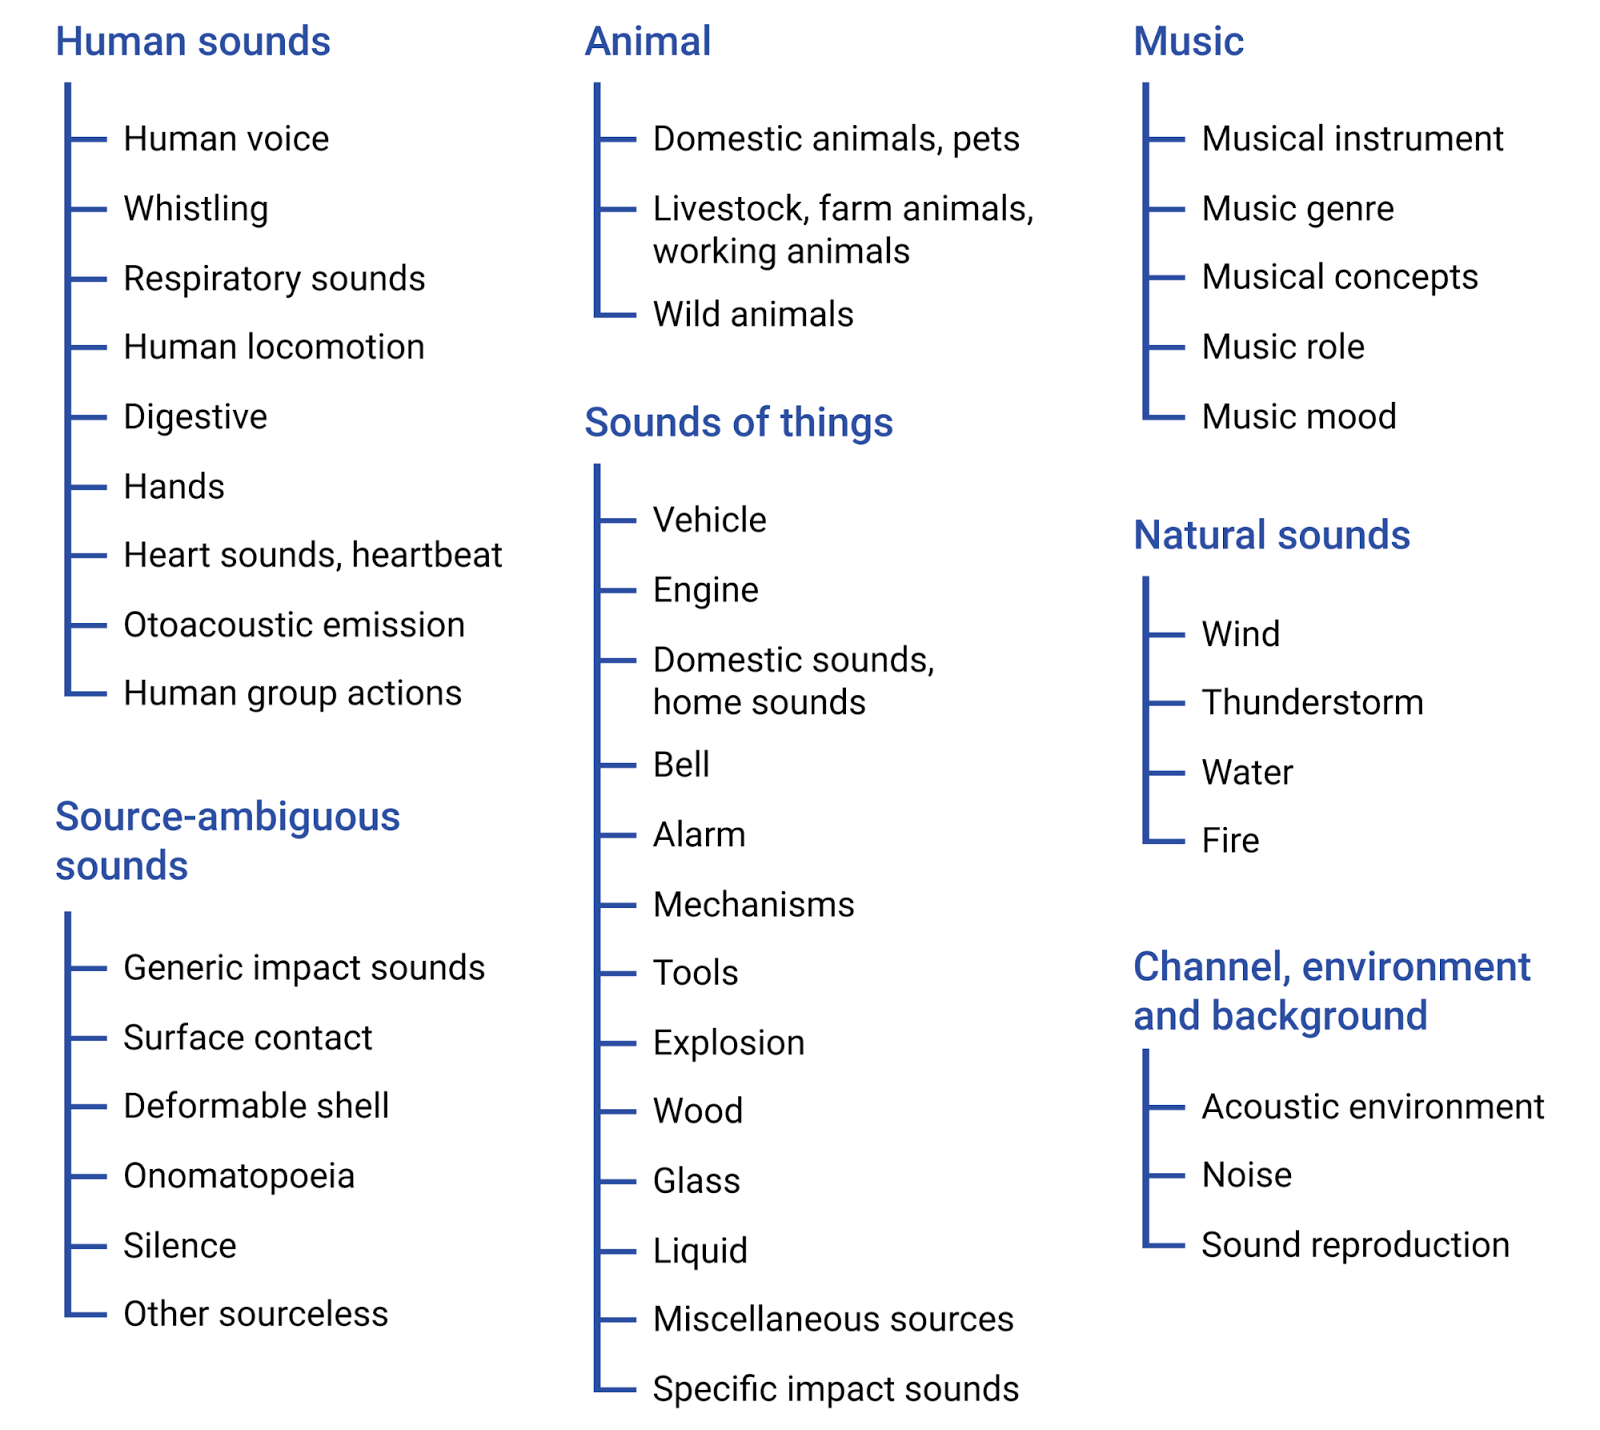
\includegraphics[scale=0.21]{audioset-ontology}
		\caption{First two layers of Audio Set Ontology}
		\label{fig:mesh1}
	\end{figure}
	
	This whole structure has been given to the user as a file in JSON format. A couple of fields have been included for each label in order to describe its meaning and make clear its position within the hierarchy. A description for all of these can be found in table \ref{table:2}. 
	% !TeX spellcheck = en_GB
% Ontology-fields table

\begin{table}[h!]
\begin{center}
	\begin{tabular}{|| m{7em} | m{22em} ||}
		\hline
		ID & This field includes the Knowledge Graph \acrfull{mid} that best describes the sound or its source. It is used as a primary identifier for the class. \\
		\hline
		Display name & Short name formed by one or two words that identifies the audio class. It sometimes includes a small alternative separated by a comma so it does not feel ambiguous. \\
		\hline
		Description & One or two explaining sentences so the meaning of the category is more defined. These can be extracted from Wikipedia or WordNet. \\
		\hline
		Examples & At least one example of the label is provided as a URL of a YouTube video. \\
		\hline
		Children & An array filled by the \acrfull{mid}s from all immediate children of the class. \\
		\hline
		Restrictions & It specifies if the category in question either has been discarded or there are no audio clips under it. \\
		\hline
	\end{tabular}
\end{center}
\caption{Fields per category in the ontology.}
\label{table:2}
\end{table}
	For the field \textit{ID}, the identifiers are known as \acrfull{mid} and belong to the \textit{Knowledge Graph} designed by Google \cite{Singhal2012}. This is a knowledge base that Google services use to improve the quality of its search results and it is composed with information extracted from a wide variety of sources. The \acrshort{mid}s are the identifiers of the different elements that belong to this huge dictionary. For instance, the \acrshort{mid} of the word "Speech" is "/m/09x0r". Another field that deserves a special explanation is the one corresponding to \textit{Restrictions}. Within all the categories of sound events, there are two flags that indicate an exclusive behaviour that differ from a typical label: "blacklisted" and "abstract". The former refers to a class that has been hidden from labellers due to its confusing meaning. The latter has been used for those classes that are just utilized as intermediate nodes in order to provide a better grouping inside the organization, and are not expected to be used in the implementation tasks. In total, out of the 632 categories, 56 have been categorized as "blacklisted" and 22, as "abstract".
	
\subsection{Dataset}

	The different YouTube videos that constitute the dataset are included in a CSV file in which each row is formed by the video identifier, the start and end time of the audio event within the video and the ontology labels that the certain clip belongs to. All the video segments have a longitude of 10 seconds maximum, except from those that the original video is shorter. \todo{Include any explanation about ratings?}
	
	The final release of the dataset is composed by 1,789,621 segments, with a duration of 4,971 hours of video and audio. After executing the selection process in which the different labels were populated with the final corresponding segments, a total of 527 classes were gathered, out of which 485 counted with at least 100 samples.
	
\subsection{Format available}

	The data can be obtained through the website \cite{SoundUnderstandinggroup2017} in two different formats:
	
	\begin{itemize}
		\item Files in \acrshort{csv} format that include for each video segment its YouTube video ID, start time, end time and the one or more labels it belongs to. 
		\item Instead of the audio files themselves, they provide already extracted audio features for each segment in compressed files that can be easily downloaded.
	\end{itemize}

	For our purpose, we worked with the dataset in both different ways. However, we get further with the already extracted features. These are obtained by using a model called \textit{\acrshort{vgg}ish} \cite{Hershey2017} which is inspired on the well known \acrshort{vgg} neural network \cite{Simonyan2015}. The released model has been pre trained on a preliminary version of the database YouTube-8M \cite{VideoUnderstandingGroup2017}. The features are available to the user in TensorFlow \todo{cite for TensorFlow} record files and the code for the \acrshort{vgg}ish model is also included in a public repository. \todo{include a type of introduction for vggish?}

\subsection{\acrshort{vgg}ish model}
	
	

	
	
	
	
	
	
	
	
	